\chapter{Future Work}
\label{FutureWork.ch}


The future work is distributed across four key directions:

\begin{itemize}
    \item \textbf{Training White-Box Estimators:}  
    After observing how estimation models built for a family of applications (e.g., CNNs) scale empirically to newer architectures within the family (See Chapter \ref{UseCase.ch} Section \ref{ScaleEstimator}), we extend our approach to "featurizing" the model rather than treating it as a single feature (@model). This enables better scalability and further reduces the dependency on generating even full-scale (FS) data for new models or architectures. This approach relies on high-level optimization (HLO) graphs generated by the XLA compiler in TensorFlow, which are used to create graph-based features such as node attributes and adjacency matrices.

    \item \textbf{Synthesizing High-Level Optimization Graphs for a Given Model:}  
    A key bottleneck in the white-box approach is the requirement to extract model-specific features from HLO graphs, which necessitates running the model on every architecture at least once to generate the HLO. This dependency on OSC or TACC resources for inference sample collection adds computational overhead. To address this, we explore the use of Generative Adversarial Networks (GANs) to synthetically generate HLO representations instead of extracting them from actual executions, thus mitigating this bottleneck.

    \item \textbf{Reimagining the “Intelligence Plane,” an Agentic AI for MLOps:}  
    MLOps (Machine Learning Operations) integrates DevOps principles with machine learning workflows to enable scalable, automated, and reproducible model deployment. The Intelligence Plane (IP) can act as an autonomous AI agent for MLOps, optimizing job scheduling, monitoring resource allocation, and dynamically adapting inference models based on workload changes. By integrating IP as an agent, we aim to build self-optimizing MLOps pipelines capable of automated decision-making and real-time performance tuning.

    \item \textbf{Developing an LLM for a CI MLOps Agent:}  
    We propose integrating large language models (LLMs) into the CI database and exposed APIs, creating a conversational interface for users. This interface can assist researchers by answering queries related to resource estimation, job scheduling, and cost analysis. Additionally, the LLM can explain estimation computations, provide recommendations, and help users navigate the scheduler framework. By bridging natural language processing (NLP) with CI MLOps, this approach enhances user accessibility and improves interaction with complex HPC workflows.
\end{itemize}

\section{Training White-Box Estimators}

\subsection{Background}

This section explores the relationship between computational graphs, DNN workload execution (e.g., training), and hardware-aware features for GPUs, highlighting the role of Graph Neural Networks (GNNs) in developing new white-box estimators.

\subsubsection{Computational Graphs in DNN Frameworks}

Machine learning frameworks like TensorFlow and PyTorch represent DNN models as computational graphs, where nodes represent operations and edges define data dependencies. This graph structure enhances efficiency and optimization, especially for training large models. The advent of ML compilers, such as XLA (Accelerated Linear Algebra), has refined this process by converting computational graphs into High-Level Optimizer (HLO) graphs, an intermediate representation that optimizes computational workflows. HLO graphs break down complex DNN operations into smaller, hardware-optimized tasks.  

Studies, such as TPUGraphs \cite{phothilimthana2023tpugraphs}, show that HLO graphs, particularly when deployed on accelerators like TPUs, improve performance by optimizing dependencies and memory usage. This approach informs our project, where HLO-extracted features enrich the HARP framework for more accurate runtime predictions.

\subsubsection{Hardware-Aware Prediction Models}

Recent research highlights the significance of hardware-specific features in improving resource prediction models. Prior work \cite{zhang2023gpu} has explored GPU-based predictors incorporating attributes such as memory bandwidth and core configurations to estimate DNN training performance across various GPU architectures. This hardware-aware strategy has shown substantial accuracy gains by aligning predictions with device capabilities.

Building on these insights, our approach integrates hardware features (e.g., CUDA cores, tensor cores) into the HARP framework. By incorporating these attributes, the enhanced HARP estimator produces hardware-adaptive runtime predictions, optimizing model performance on different computing infrastructures.

\subsubsection{Graph Neural Networks for Resource Prediction}

Graph Neural Networks (GNNs) \cite{kaufman2021tpu} effectively model complex relationships within computational graphs, making them well-suited for resource prediction in DNN workloads. By capturing hierarchical and sequential dependencies, GNNs provide a more structured representation of computational flow than traditional approaches.

GNN-based models have been successfully applied to TPU-inspired resource prediction frameworks, where they embed node features and adjacency information for improved runtime estimation. Our project leverages GNNs to model DNN computational flows extracted from HLO graphs, enabling the extended HARP framework to generalize across different DNN architectures and adapt to diverse hardware configurations.


\subsection{Methodology}

We configure the HARP framework with an enhanced data capture pipeline, enabling the generation of training data while extracting new features from HLO graphs. Figure X outlines these newly captured features, encompassing both model-specific and hardware-specific attributes, which contribute to building HLO-based white-box estimators.


\begin{figure}[ht]
    \centering
    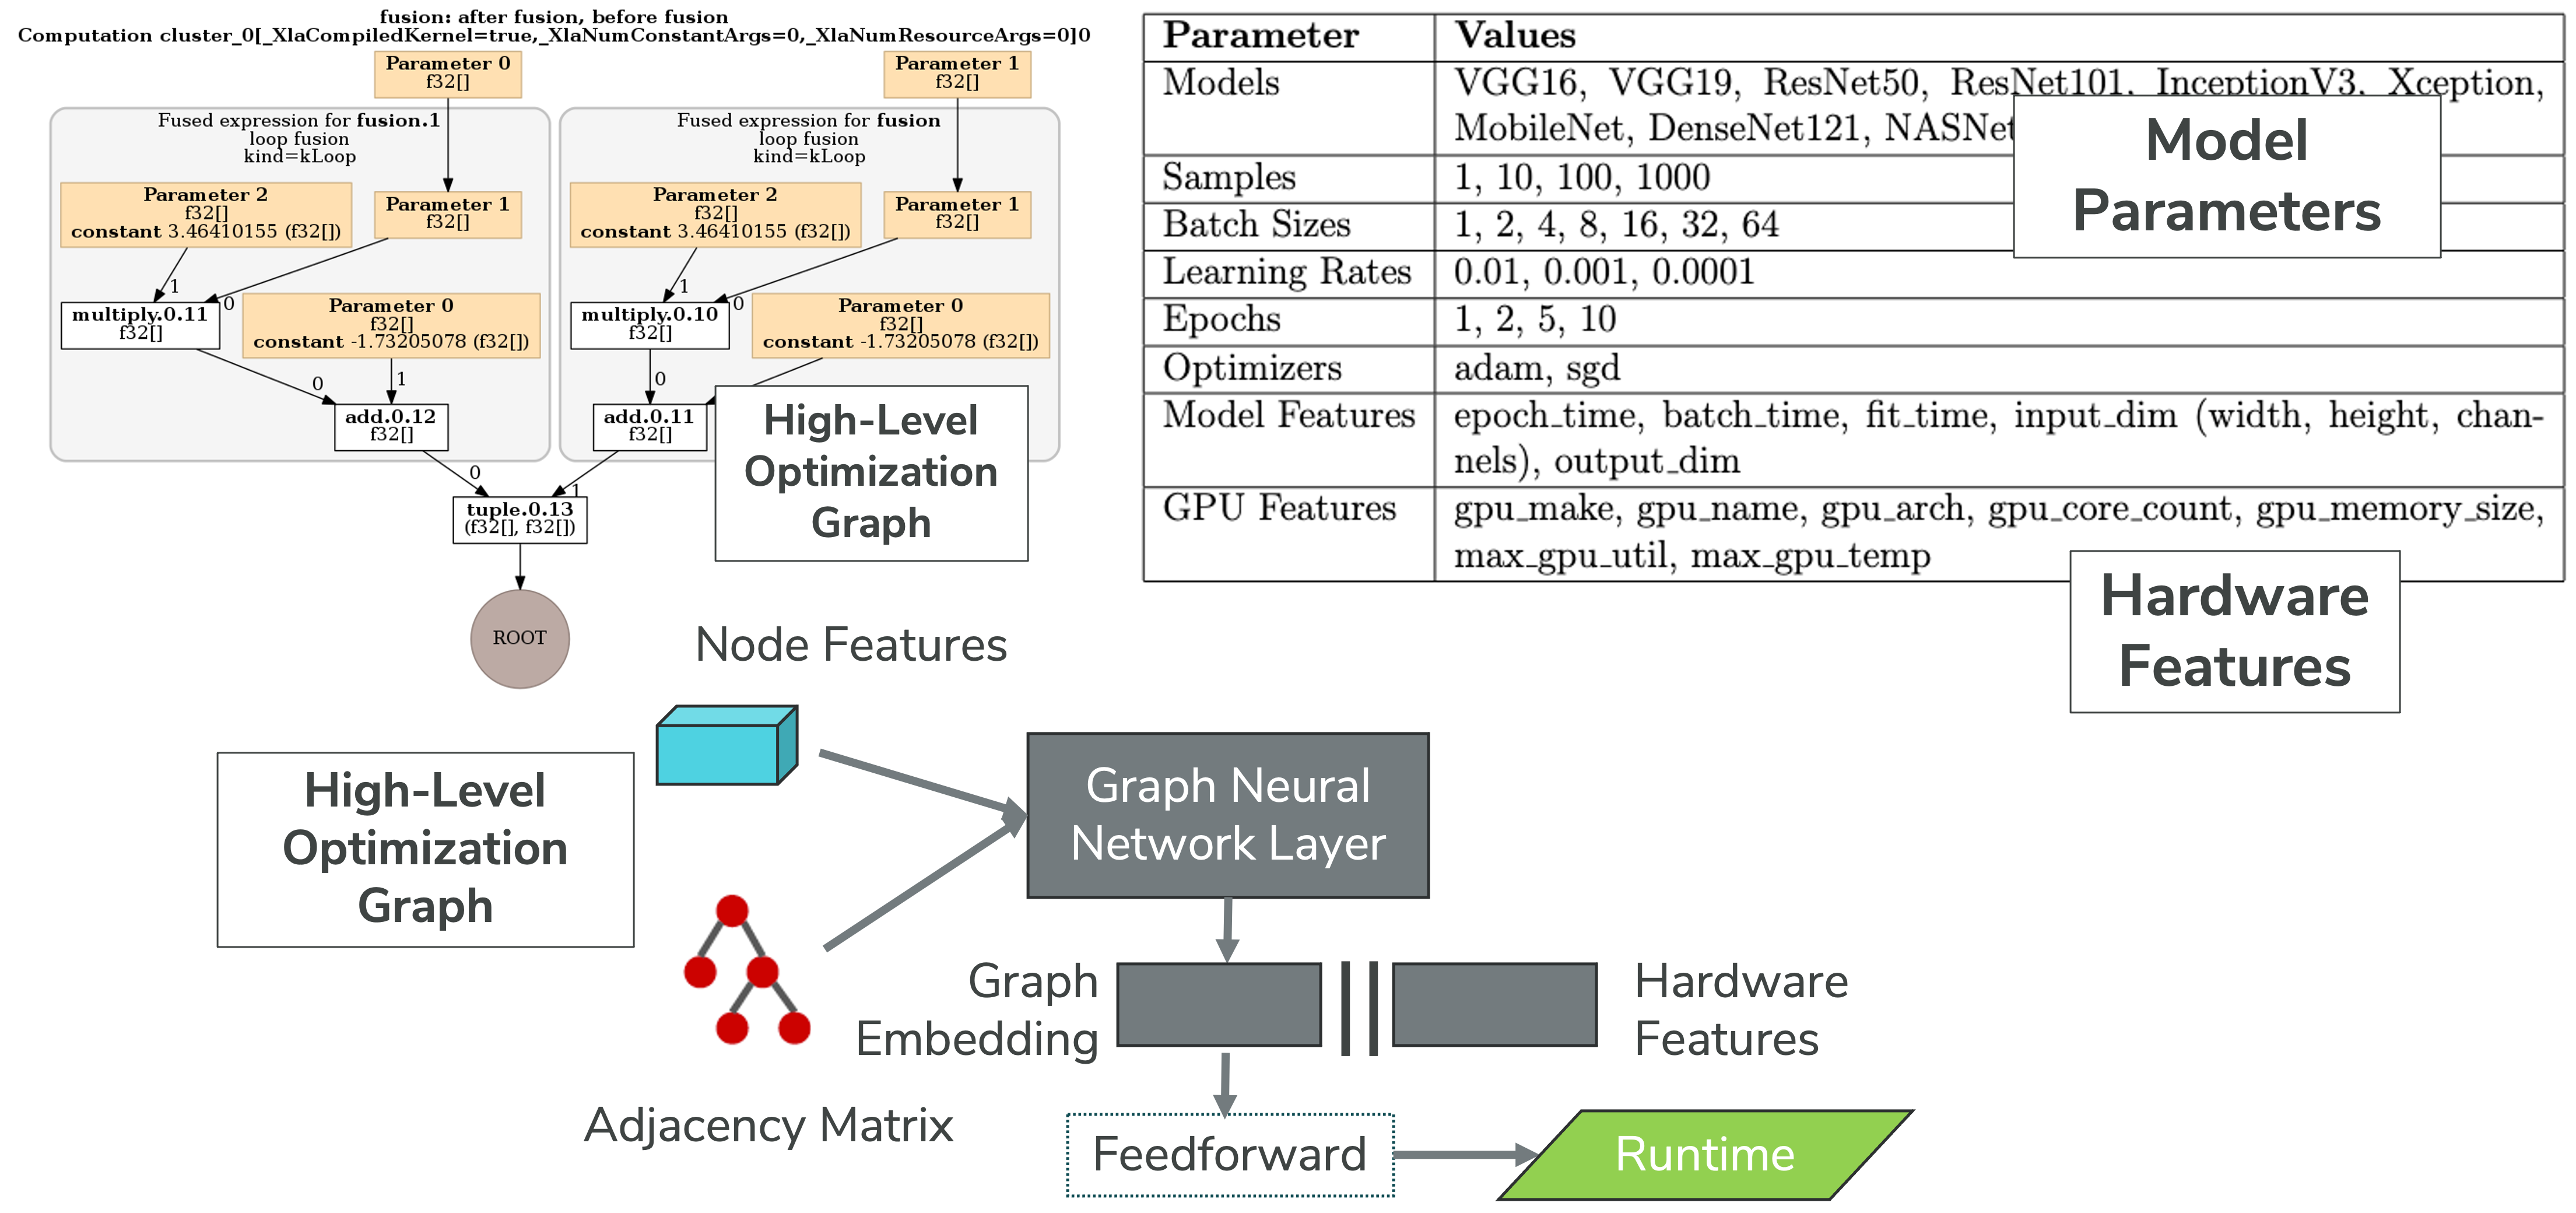
\includegraphics[width=\textwidth]{Images/WhiteBox.png}
    \caption{Feature extraction using High-Level Optimization (HLO) graphs for training white-box estimators.}
    \label{fig:HLO_WhiteBox}
\end{figure}

\subsubsection{Dataset Description}

Our dataset consists of over 20,000 records, each representing a unique configuration across model architectures, GPUs, and hyperparameters. Data collection was conducted across three Ohio Supercomputing Center (OSC) clusters: Owens (Nvidia P100), Pitzer (Nvidia V100), and Ascend (Nvidia A100). The dataset comprises 30 distinct features, covering input-output specifications, GPU-specific attributes, and model performance metrics, as detailed in Table \ref{table:dataset_features}. Additionally, it includes NPZ files generated using a new feature capture pipeline, which extracts High-Level Optimization (HLO) graphs and features from computational workloads \cite{kaufman2021tpu}. 

\begin{table}[h!]
\centering
\resizebox{\textwidth}{!}{%
\begin{tabular}{|l|p{4cm}|p{8cm}|}
\hline
\textbf{Feature} & \textbf{Type} & \textbf{Description} \\
\hline
Name & Identifier & Unique identifier combining model, optimizer, sample size, input dimensions, and parameters \\
\hline
samples & Integer & Number of samples used for each configuration \\
\hline
input\_dim\_w, input\_dim\_h, input\_dim\_c & Integer & Input dimensions (width, height, channels) \\
\hline
output\_dim & Integer & Number of output classes \\
\hline
epochs & Integer & Number of training epochs \\
\hline
batch\_size & Integer & Training batch size \\
\hline
learn\_rate & Float & Learning rate for optimization \\
\hline
tf\_version & Categorical & TensorFlow version for reproducibility \\
\hline
cuda\_version & Categorical & CUDA version used by TensorFlow \\
\hline
batch\_time & Float & Time taken per batch \\
\hline
epoch\_time & Float & Time per epoch \\
\hline
fit\_time & Float & Total training time \\
\hline
npz\_path & String & Path to associated NPZ file \\
\hline
gpu\_make, gpu\_name & Categorical & GPU manufacturer and model \\
\hline
gpu\_arch & Categorical & GPU architecture (e.g., Ampere for A100) \\
\hline
gpu\_cc & Categorical & GPU compute capability \\
\hline
gpu\_core\_count & Integer & Number of CUDA cores \\
\hline
gpu\_sm\_count & Integer & Number of streaming multiprocessors \\
\hline
gpu\_memory\_size & Integer & GPU memory size (GB) \\
\hline
gpu\_memory\_type & Categorical & Type of GPU memory (e.g., HBM2e) \\
\hline
gpu\_memory\_bw & Integer & Memory bandwidth (GB/s) \\
\hline
gpu\_tensor\_core\_count & Integer & Number of tensor cores \\
\hline
max\_memory\_util, avg\_memory\_util & Float & Maximum and average GPU memory utilization (\%) \\
\hline
max\_gpu\_util, avg\_gpu\_util & Float & Maximum and average GPU utilization (\%) \\
\hline
max\_gpu\_temp, avg\_gpu\_temp & Float & Maximum and average GPU temperature (\degree C) \\
\hline
\end{tabular}%
}
\caption{Dataset Features with Descriptions}
\label{table:dataset_features}
\end{table}

\paragraph{NPZ File Details}

Each dataset entry is associated with an NPZ file containing fine-grained computational graph data extracted from HLO graphs. The following key feature groups are included:

\begin{itemize}
    \item \textbf{Node Features}: Descriptive properties for each node in the computational graph:
        \begin{itemize}
            \item \textbf{Root Indicator (is\_root)}: Identifies the final output node.
            \item \textbf{Tensor Type Encoding}: One-hot encoded representation of tensor data types.
            \item \textbf{Tensor Shape Features}: Includes shape dimensions (up to six), sum, and product.
            \item \textbf{Convolutional Operations}: Window size, stride, padding configurations.
            \item \textbf{Slice & Dynamic Slice Features}: Range indicators and slice sizes.
        \end{itemize}
    \item \textbf{Tile Configuration Features}: Defines tiling strategies for optimizing convolutions.
    \item \textbf{Layout Configuration Features}: Specifies memory layout strategies for tensors.
\end{itemize}

\paragraph{Dataset Generation}

Data was generated by systematically varying hyperparameters such as sample size, batch size, learning rate, epochs, and optimizers across 17 different models. Figure \ref{fig:dataset_parameters} outlines the range of model and hardware parameters captured within the dataset.


\section {Reimagining the “Intelligence Plane” an Agentic AI for MLOps:}

\subsubsection{MLOps Overview}

MLOps (Machine Learning Operations) is a set of practices designed to streamline the development, deployment, monitoring, and automation of machine learning (ML) models in production environments. It integrates principles from DevOps, Data Engineering, and ML Lifecycle Management to ensure scalability, reproducibility, and reliability of ML workflows.

\paragraph{Key Components of MLOps}
This section outlines the core components of MLOps and how ICICLE components support and implement these functionalities.
\begin{itemize}
    \item \textbf{Model Development \& Versioning} – Managing code, data, and model versions for reproducibility. (Handled by \textbf{Model Commons})
    \item \textbf{Automated Training \& Testing} – Continuous retraining using CI/CD pipelines. (Using \textbf{HARP} and \textbf{iScheduler})
    \item \textbf{Model Deployment \& Serving} – Deploying models in production using Kubernetes, Docker, or cloud services. (Using \textbf{TAPIS})
    \item \textbf{Monitoring \& Performance Tracking} – Observing model drift, latency, and performance metrics. (Using \textbf{Kafka} in the \textbf{Smart Scheduler Framework})
    \item \textbf{Feature Engineering \& Data Management} – Ensuring high-quality data pipelines. (Customizable by users, enabled by \textbf{TAPIS Workbench})
\end{itemize}

MLOps facilitates seamless collaboration between data scientists, engineers, and IT teams, ensuring robust and efficient AI model lifecycle management in production.

\subsubsection{ICICLE Intelligence Plane Overview}

The ICICLE Intelligence Plane is a federated subsystem that governs performance metrics, resource allocation, and AI-driven workflows within the ICICLE ecosystem \cite{panda2024creating}. It facilitates the construction, deployment, and optimization of intelligent components, including machine learning models, middleware, runtime schedulers, and resource estimators.

\paragraph{Key Components of the Intelligence Plane}
\begin{itemize}
    \item \textbf{Smart Scheduler} – Estimates training times, evaluates queue conditions, and schedules jobs for optimal execution.
    \item \textbf{Edge Trigger Mechanism} – Monitors model accuracy and triggers retraining events based on predefined thresholds.
    \item \textbf{HARP Pipeline} – Optimizes resource allocation when estimator performance declines.
    \item \textbf{Job Progress Monitor} – Tracks job execution and provides real-time updates on model training and deployment.
    \item \textbf{Model Cards} – Documents and registers new models (e.g., smaller architectures, improved versions) for reproducibility and transparency.
    \item \textbf{Event Handling Framework} – Detects and processes key retraining and execution events:
    \begin{itemize}
        \item New data availability.
        \item Insufficient images in the observation folder.
        \item Job execution status updates.
        \item Model accuracy drops below a predefined threshold over $N$ inferences.
        \item Health check failures in estimation models.
        \item New model registration triggers (e.g., smaller models, new architectures).
    \end{itemize}
    \item \textbf{Rules Database} – Stores and maintains monitoring policies:
    \begin{itemize}
        \item Tracks applications and their performance metrics (accuracy, energy consumption, etc.).
        \item Stores model metadata in \textbf{Data Commons} while summarizing statistics in \textbf{Component Commons}.
    \end{itemize}
    \item \textbf{Watch Folders} – Continuously monitors new training data (e.g., images from edge devices) to trigger automated processing.
    \item \textbf{Service Orchestration Engine (Daemon Endpoints)} – Manages job scheduling, execution monitoring, and system performance tracking:
    \begin{itemize}
        \item \textbf{Job Monitoring Daemon} – Uses \textbf{SLURM} and \textbf{Kafka} to monitor job performance and update the \textbf{Component Start Database}.
        \item \textbf{Estimator Health Checker} – Periodically validates the accuracy and efficiency of estimation models.
    \end{itemize}
    \item \textbf{Training Data Generation Module} – Expands training datasets by running phase-one \textbf{HARP-return models} in new environments or integrating updated versions (e.g., MDv5, MDv6) into the training pool.
\end{itemize}

\begin{figure}[]
    \centering
    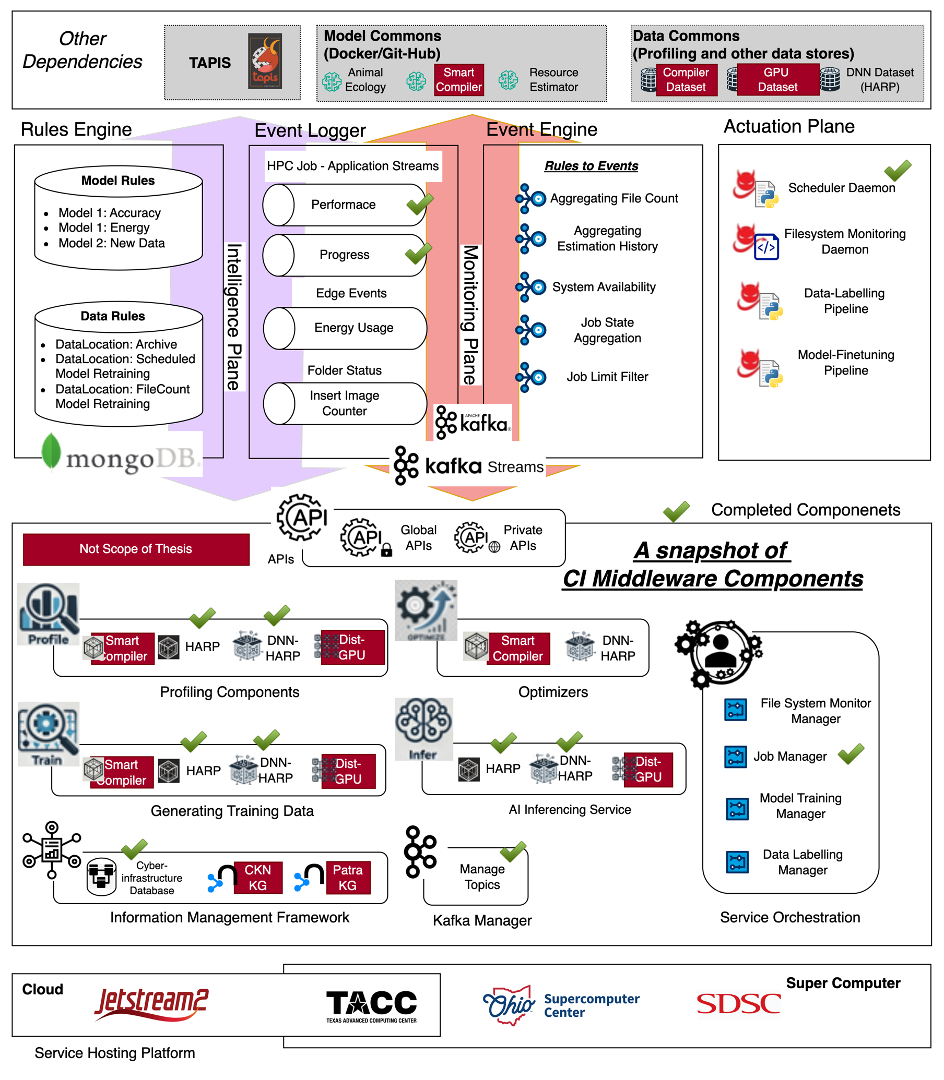
\includegraphics[width=\textwidth]{Images/IPv2.png}
    \caption{Overview of CI Middleware Components and Workflow in the ICICLE Intelligence Plane. The diagram illustrates key components, including data and model commons, monitoring and intelligence planes, profiling and optimization frameworks, and service orchestration across cloud and supercomputer environments.}
    \label{fig:ICICLE_CI_Middleware}
\end{figure}


The ICICLE Intelligence Plane facilitates a fully automated, AI-driven scientific workflow, incorporating model retraining, event-driven execution, and real-time performance monitoring to enhance adaptability and efficiency across various research applications. Figure \ref{fig:ICICLE_CI_Middleware} illustrates the current implementation of the Intelligence Plane alongside the proposed Intelligence Plane v2.0 architecture.

\subsubsection{Intelligence Plane as an Agentic AI for MLOps}

Agentic AI refers to AI systems that autonomously perceive, reason, and act to achieve specific goals with minimal human intervention. Unlike traditional AI, which passively processes inputs, Agentic AI actively interacts with its environment, makes adaptive decisions, and refines its behavior over time.

\paragraph{Key Components of Agentic AI and ICICLE’s Alignment}
\begin{itemize}
    \item \textbf{Perception Module} – Gathers real-time data from sensors, databases, or APIs. (Implemented through \textbf{Watch Services, Edge Triggers, Job Monitors, and CKN} \cite{withana2023ckn})
    \item \textbf{Reasoning \& Decision-Making} – Utilizes symbolic reasoning, reinforcement learning, or planning algorithms.
    \item \textbf{Action Execution} – Takes autonomous actions based on learned strategies. (Enabled via the \textbf{Service Orchestration Engine})
    \item \textbf{Feedback Loop \& Adaptation} – Continuously learns from past actions to improve future decisions. (Orchestrated via \textbf{CKN} and other monitoring tools in collaboration with the Rules Engine and trigger handlers such as the Edge Trigger Mechanism.)
    \item \textbf{Goal-Oriented Behavior} – Aligns actions with long-term objectives through self-improving mechanisms. (Defined by the Rules Engine, e.g., setting accuracy thresholds for the \textbf{Animal Ecology Use Case} or dynamically optimizing resource estimators.)
\end{itemize}


\subsection{Use Cases}

As part of future work, we aim to leverage the new Intelligence Plane - Agentic AI for MLOps to orchestrate an end-to-end workflow for animal ecology model training and deployment. This will involve integrating various ICICLE components while incorporating modular elements of HARP and iScheduler. By doing so, we seek to enable adaptive estimators that can generalize to new models or enhance accuracy based on historical data and available computational resources.



\subsubsection{Use Case 1 - Animal Ecology}

The invoker initiates the workflow by setting up the Edge Simulation, using the provided code repository from GitHub (\url{https://github.com/tapis-project/camera-traps}). The process begins with preparing the Edge Device Image and determining whether an image is out-of-distribution (OOD). If an OOD event is detected, it is stored in CKN and streamed via Kafka, where it undergoes rule-based filtering to assess if it meets OOD criteria.

Once the Monitoring Plane (MP) validates an OOD detection, it triggers the Retraining Event via CKN. At this stage, the Rule Engine reads predefined parameters to define necessary inputs for action. This includes:
\begin{itemize}
    \item Selecting the appropriate model for retraining.
    \item Retrieving stored model weights.
    \item Identifying the location of labeled training datasets.
    \item Determining training parameters – either default settings or Hyperparameter Auto-Tuning (HPA).
\end{itemize}

Next, the Intelligence Plane (IP) assigns the retraining task to the Smart Scheduler (SS) Pipeline, which handles execution by:
\begin{enumerate}
    \item Fetching available systems from the database.
    \item Performing resource estimation using inference models and CKN inputs.
    \item Checking queue availability via TAPIS.
    \item Selecting the fastest system with optimal runtime and queue availability before submitting the job.
\end{enumerate}

Once submitted, the Job Daemon continuously monitors execution, tracking job status, verifying if it will complete within the allocated time, and ensuring successful completion.

Upon completion, the Model Retraining Pipeline updates the trained model version, stores it on Hugging Face, and updates the corresponding Patra Model Cards for documentation and deployment. Throughout the process, Sachith and Neelesh oversee critical aspects of the Intelligence Plane’s execution and model storage, ensuring efficient scheduling and deployment.


\subsubsection{Use Case 2: HARP - Adaptive Estimation Refinement}
In Chapter \ref{BuildEstimator.ch}, we explored how the availability of new data (as shown in Figure \ref{fig:data_availability_pattern})  facilitates retraining estimators to adapt to new environments (e.g., a new cluster). Building on this, we leverage the existing HARP and Intelligence Plane (IP) framework (depicted in Figure \ref{fig:HARP_pipeline}, \ref{fig:iScheduler}) to establish a workflow similar to the Animal Ecology use case. This workflow is triggered by estimation errors (e.g., misestimations for MegaDetector) to retrain the MegaDetector estimators and deploy updated models for improved inference in future executions.


